\chapter{Formulation}
% comit 21-11-2017
\minitoc
%The following chapter is focused on the problem formulation for cameras positioning.\\
%Obviously formulation proposed in not the only one and some other have been proposed in the literature, mostly depending then the objectives. \\
The formulation of the problem is essential in order to design an efficient cost function. The cost function is  used to quantifies the quality of the solutions. It is a crucial element for the optimisation processes.\\
This chapter present first, a formal definition  of the problem based on the literature and in the second time our formulation is proposed. The formulation proposed is  adapted to the problems of efficient coverage using camera mounted on UAV.

\section{ Coverage estimation. }


 The question in this section is to estimate the covered area depending then the cameras pose.\\

%What should be control by the video surveillance? \\
%One aim of the video surveillance is to detect some anomaly in the area for that the number of black hole need to be reduce. A black hole is zone not cover by the system of video surveillance. Estimate the part cover by the system of video surveillance is primordial to limit the size and the number of black hole. 
%To know if the area is cover by a minimum of one vision sensor, different techniques can be used.
%Indeed the coverage estimation is essential element to optimise the position of a network of cameras. But before to find the position some assumption should be done to describe our problems and explain the methodology to calculate the coverage rate of an area.
%The main purpose of our work is to estimate the position for the vision sensors network into a given area.\\
%Where the main goal is to manage the positioning of the fix number of cameras in order to maximize the visual coverage. 
%Indeed before to find the position some assumption should be done to describe our problems.\\ 

The term coverage denote the area visible by at least one camera. Also the area to cover represent all the area which must be control by at least one camera. 

Therefore the problem is formulated as:
\begin{itemize}
\item [-] Maximization of the coverage with a fix number of cameras.
\item [-] Minimization of the constraints.\\  where the constraint can be for examples the complex shape of the area, the bound of the area, the altitude of the cameras,...
\end{itemize}

%The problem needs to be formalized in order to clearly identify the complexity of the cameras positioning. 


Due to this formulation, composed by the maximisation and minimization, the solution  have to evolve to a best  possible answer based on the cost function. Depending then the formulation of the area and the design of the cost function the ability to optimize a solution is greatly affected. 
The positions of the cameras have to limit the number and the size of black
holes to be exploitable. The black holes are the area not covered by the camera
views. To do so a precise estimated of the part covered by the system of camera views is elemental.\\


In order to estimate the coverage properly the area must be discretized. Once the area discritezed it became easier to verifies if each point of the area are coverer by at least one camera of the network.
%The coverage problem must be modelled properly. The different method to design the problem will affect the solution and the applicable resolve method. The following part will talk about it \\
%The coverage problem must be modelled properly. The different method to design the problem will affect the solution and the applicable resolve method. \\
%The first part is to estimate properly the coverage of the area. To do so many method have been developed most of them are based on the occupation grid $G$ of the area. \begin{equation}
%G=\begin{bmatrix}
% g_1 ...g_i ... g_m
%\end{bmatrix}  , m\in \mathbb{N}
%\end{equation}
%Where $m$ is the number of points in the grid.
%The occupation grid is mostly placed on the floor of the area to cover. At minima each point $g_i$ of the grid $G$ should be cover by the vision sensors. Consequently a list of points is created to listed the covered part of $G$ which are noted as $Pc$.
%\begin{equation}\label{eq:Pci}
%g_i \in Pc \mbox{ IFF } g_i \mbox{ is coverd. }
%\end{equation}
%
%The modelization of the grid is an important element and different solution has been proposed during the time with different advantage depending then the situation.\\

\subsection{Grid}


%/!$\backslash$ \textbf{ ajouter une partie dedier  a [181*] qui propose une solution pour ajusté la densité en fonction  de la necesité de présision  (contour plus dense ) }

The first part is to estimate properly the coverage of the area. To do so many method have been developed most of them are based on the occupation grid $G$ of the area. 
\begin{equation}\label{eq:Grid}
	G=\begin{bmatrix}
	 	g_1 ...g_i ... g_m
	\end{bmatrix}  , m\in \mathbb{N}
\end{equation}
Where $m$ is the number of points in the grid.
The occupation grid is placed on the area to cover. At minima each point $g_i$ of the grid $G$ should be cover by a cameras. Consequently a list of points is created to listed the covered part of $G$ which are noted as $Pc$.
\begin{equation}\label{eq:Pci}
g_i \in Pc \mbox{ IFF } g_i \mbox{ is coverd. }
\end{equation}


The modelization of the grid is an important element and different solution has been proposed during the time with different advantage depending then the situation.\\

\subsubsection*{Related work for the grid design}
The following subsection is focused on the different  modelling the grid possibility, based in the literature. 

\paragraph*{ Sampling frequency} %Sampling frequency.\\
The occupation grid is use to discretize the area to cover. The discretization of the area can vary and the area can have a high level of discretization or low level. 
The high level of discretization or high sampling frequency of an area is characterized by a big amount of point $g_i$ for the area. The hight sampling frequency have to consequence to have important density of point $g_i$ and the value of $m$ is high. 

%\begin{equation}
%	G=\begin{bmatrix}
% 		g_1 ...g_i ... g_m
%	\end{bmatrix}  , m\in \mathbb{N}
%\end{equation}
%
%Where m is the number of point into the grid.
 
The advantage to have a high sampling frequency is to have a better estimation of the coverage. More the discretization is high more the estimation of the coverage will be sharp. In [171*] an example of high frequency sampling is given. 
In [22*] the points of interest called targets are the points to cover. These targets are the goals and the optimization is focus on cover the maximum of this targets. In [22*] Zhao et al change the number of target to have a better result. Increasing the frequency of point in order to refine the solution and add more cameras for a better coverage of the area.  \\
In fact the quality of the coverage estimation affect the positioning optimization. %A bad estimation of the area coverage due to the bad level of discretization will impact the quality of the answer and the precision of the cameras position by returned a approximate coverage rate. 
A bad estimation of the area coverage due to the low density of point in the grid will give an approximate view of the area covered and some black hole can appear during the optimisation process. This black hole can be too small to be detected because of the low density of point. 
% the quality of the coverage will be approximate. 
\\
On another side the disadvantage to have a too high sampling frequency is the time computation. Rather to refine the solution the too high level of discretization of the area will make the optimization too long and more complex. Indeed to control the coverage is necessary to control if each point of the area is covered by a cameras.  
\begin{equation} 
	\sum^m \sum^n \mbox{test of coverage}
\end{equation}

Where $m$ is the number of point in the grid and $n$ the number of camera.  More the size of the grid is high more unity test of coverage (defined later see in section \ref{sec:CamerasCoverage}) should be done at each step of the optimization process. During the optimization the size of the grid will greatly affect the time computation.  \\

Also the frequency sampling is often link to the pose precision of the camera and the size of the search space. The search space represent the domain to optimize or can be defined by the set of all possible solutions in our case the search space is all the position for all the cameras. 
Therefore increase the number of point in the grid will also increase in proportion the number of position possible for each cameras. The too high precision in the position of the camera will increase the complexity and some case where the value of $m$ is too high the optimization process cannot converge or find acceptable solution to the gain of the search space. \\ 

At the opposite a lower  frequency can be a good solution to upgrade the convergence speed of the optimization process as that was presented in [8*] where a small value of $m$ and the optimization of the problem formulation has been proposed to have a real time solution for small area and just few cameras ( up to  20).\\

The too low sampling frequency instead to win  computation time, may affect the quality of the answer. In fact as the previous part explain the impact of a too high frequency in the solution, a too low impacted the pose of the camera by have a wrong or bad estimation of the coverage.  \\
The density of the grid need to be adjusted depending then the goal and the precision required. One of the solution proposed in Zhao et al[22*] is to progressive refinement in grid density.

\paragraph*{ Distribution}
The distribution is an important factor to manage for design an occupation grid. The distribution is the method applied to describe the area to cover by the position of each point $g_i$.
Different distribution can be use but commonly in the literature the grid pattern distribution and in a lesser extent the random distribution is applied (see Figure \ref{fig:GridVsRand}). \\
\begin{figure}[t!]
\minipage{0.65\textwidth}
   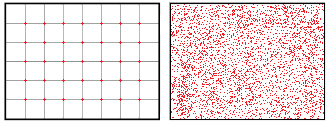
\includegraphics[width=\linewidth]{img/GridVsRand.png}
  \caption{ (a)Grid with uniforme and regular distribution.\\   
(b) Random distribution.\\  
}\label{fig:GridVsRand}
  \endminipage\hfill
\end{figure}
The random distribution is less popular but it is used in [22*] in order to reduce the number of point in to the uniform grid pattern while maintaining the quality of the solution. In this case the random is use to select randomly the target when the precedent frequency of the grid was too high. So as to reduce size of the grid a random selection of the point of the grid is used. \\
The solution proposed in [22*] is quiet specific. In the [83*] [171*] the random distribution is use to describe the area to cover. \\
In Hoster et al [171*] the point of the grid are randomly distributed to describe all the area to cover. The advantage on this article is to use the random distribution in order to  manage the density of point in some specific region of the area. Especially By increasing the density of point on some specific zone of the area. the density increase allows to give more importance to this zone (see Figure \ref{fig:randomGridRef171})\\
Indeed the higher density will affect the optimization process and the area with more density will be comparatively  more profitable to a low density area. The highest density will be cover in priority despite to an insufficient amount of cameras. This mechanism is even simplified due to the random distribution.

%%%%% FIGURE  random distribution  form 171*
\begin{figure}[t!]
\minipage{0.65\textwidth}
   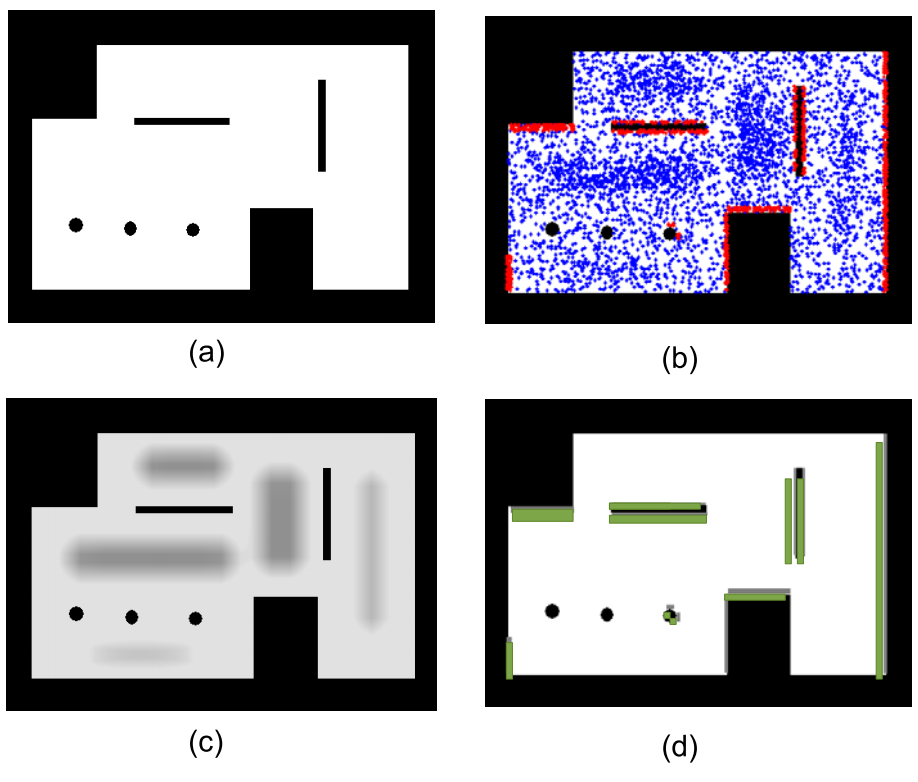
\includegraphics[width=\linewidth]{img/randomGridRef171.png}
  \caption{ (a )area  to cover.\\   
(c) Importance of the area.\\  
(b) grid representation.}\label{fig:randomGridRef171}
  \endminipage\hfill
\end{figure}

The hengel et al [83*] have test the random distribution and the uniform grid pattern distribution before to conclude the grid pattern and the random distribution propose globally the same result, when there is no priority zone in the area. Based on this observation hengel et al [83*] decide to use the uniform grid notably because of its simplicity of implementation.\\

\paragraph*{ Special modelization (3D  or 2D)}
To design the occupation grid one other element should be taken in consideration, it is the spacial modeliszation. After deciding the useful density and the distribution of the grid, the position in the space of the point $g_i$ need to be studied.   %After the distribution of the grid, the special modelization is studied. 
In fact depending then the problem the grid can be modelled differently in order to cover properly some specific region of interest. Commonly  the occupation grid is placed on the floor and calculate visibility only in 2D  [164*][150*][8*][170*][171*][22*] but depending then the context the grid have interest do describe a 3D space or a specific region.  
Hegle et al[83*], calculates the visibility where it is relevant: for example, on the upper torso or head of the possible target rather than the floor. This article  propose a 2D grid but inside the 3d space in order to  characterize properly the volume by placing the grid at specific height.  \\

In [82*] the grid is formalized in the full volumetric space by numerous “control Point” (as $g_i$) for control the area. The point of the grid are uniformly (or can be randomly) distributed along the axis of $x, y$ and $z$. Also in [87*] the grid are formulated in the volumetric space by using a uniform 3D grid distribution. The formulation proposed show the complexity even more important to use a 3 dimensional occupation grid and for practical reasons (mostly the inadequacy has computational power due to the increased complexity) the 3D grid is replaced by a 2D grid at a specific height to optimize the coverage. \\ 
While an occupation grid designed to estimate the volume to cover along the $ x, y $ and $ z $ axes of the area already exists and his implementation is unusual due to the increasing complexity for the optimization process.  
Nevertheless some solution was discussed [141*] [83*] to take into account the vplume of the area to cover which cannot be only limited to an occupation grid along the axes $ x $ and $ y $as a simple 2d grid placed on the floor.\\
In [83*] is focus on estimate the area to cover inside a 3 level building. To estimate the coverage in the building the grid was placed at all the level. This solution is efficient in order to limit the number of point in the grid compare then a full volumetric description of the area and keep the 3 dimensional information by adding one layer for each level of the building.  \\
The 3 dimensional grid can be exploit not only in term of described a volumetric space, as proposed before but also in term of relief on the map. 
In [141*] propose a 2 dimensional grid adapted to the relief of the area to cover. This article are focused on cover a large outside area with an important relief. To estimate properly the area to cover a grid has been placed following the altitude of the relief. The area to cover is discretize by square of the grid with different altitude as Figure\ref{fig:grilleRef141}. Every square is use to describe the area to cover by a network of cameras.  


%%% figurir  from 141*
\begin{figure}[t!]
\minipage{0.65\textwidth}
   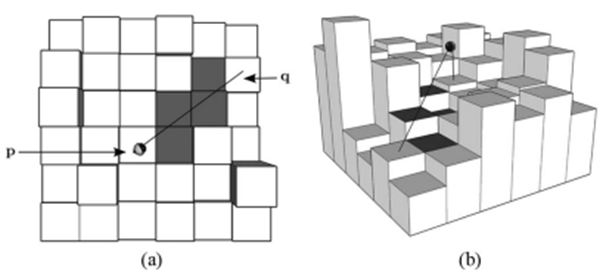
\includegraphics[width=\linewidth]{img/grilleRef141.png}
  \caption{ Relief grid use to discretize  an area with taking in account the relief  .}\label{fig:grilleRef141}
  \endminipage\hfill
\end{figure}

\paragraph*{ Zone of interest } 
The zone of interest can be design by different manner depending then the goal. Manly 3 method can be discern.
\begin{itemize}
	\item[-]	The multi coverage zone 
	\item[-]	The priority zone  
	\item[-]	Obstacle in the area
\end{itemize}
 
This 3 method to design a zone of interest are not fully independent and can be associate in the same model [141*, 171*,84*].\\ 

The multi coverage zone have to aim the control of a specific zone of the area by multiple cameras.  The multiple coverage may be called k coverage as in [174*]. Where k is the number of camera useful to cover this a zone. \\
Every points of the grid $G$ should be covered at least by one camera and for some specific zone of the area by $k$ cameras.\\
 Consequently a binary list of points is created to count the covered part of $G$ which are noted as $Pc$.

\begin{equation}\label{eq:PciK}
Pc_i= \begin{cases} 1, & \mbox{if } g_i\mbox{ is covered by $k_i$ cameras} \\ 0, & \mbox{otherwise}   \end{cases}k_i \in K
\end{equation}
Where $k_i$ is the number of camera use to cover the point $g_i$ of the grid. $K $ is the list of $k_i$ useful to cover the area associate to the point of the grid $g_i$ as in [82*]. \\%ajouté les reference 82 + kcoverage appellation.\\

The priority zone are the zone to cover in priority especially in the case where the number of cameras are not sufficient to fully cover the area. This priority of coverage can be expressed by different way. \\
In the case where the grid is uniformly distributed a weighting may be fixed on the zone of the area to cover in priority [141*,84*]. This method was implemented in [141*]  to optimize the position of the camera on the road passing through the area to cover. \\
In [171*] the weighting on the zone of interest is not did it on the point of the (uniform) grid. Instead the weight is done by increasing the frequency of point of the random grid distribution as in Figure \ref{fig:randomGridRef171}(b). Using this method the zone of interest are more dense and that push the optimization process to cover this area in priority (more density mean more interest on the cost function).\\
The priority zone in the uniform grid distribution can be formulate as: 
  \begin{equation}\label{eq:PciP}
Pc_i= \begin{cases} 1*p_i, & \mbox{if } g_i\mbox{ is covered and  $p_i$ is the weight} \\ 0, & \mbox{otherwise}  \end{cases}
\end{equation}
Where $p_i$ is the weight of the point $g_i$ on the grid $G$. $P $ is the list of $p_i$ useful to the weighting of the area associate to the point of the grid $g_i$. \\

Obstacle in the area, are the zones without interest. This zone are not strongly prohibited. That mean the zone considering as obstacle can be covered but their coverage or un-coverage does not affect the estimation of the coverage of the area. In the case of random grid distribution the obstacle zone have a frequency of control point null [141*]. For the uniform grid distribution the obstacle zone are remove to the list $Pc$. This method are currently used like in [22, 170, 141, 171, 84].

\paragraph*{Atypical design}  

We saw previously the method to set up a classical occupation grid depending then the problem. Few other solution more atypical have been developed. On solution coming from the field of wireless sensor network is the topologies grid. 
 The topologies grid is clearly explained in Chakraborty et al[150*] the interest of this  methodologies is to reduce the number of point to cover, not related to the resolution wished  but by the sensor range. Indeed the size between the point of the grid has been defined by the size of the minimal range of the sensors thank to the relation of the point are defined as a topological relation. 
Another atypical solution is to develop a grid composed by rectangles. Each rectangles may have different size adapted to the obstacle in the area. A rectangle is considered as covered if most of the area of the rectangle is cover by the cameras[170*]. This method is adapted to the area with obstacle as is show in the Figure \ref{fig:from170}
\begin{figure}[t!]
\minipage{0.65\textwidth}
   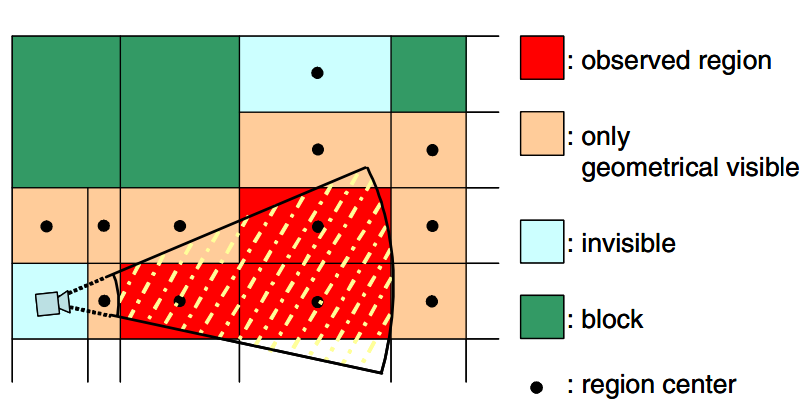
\includegraphics[width=\linewidth]{img/from170.png}
  \caption{ Observed regions from camera candidate.}\label{fig:from170}
  \endminipage\hfill
\end{figure}

\newcolumntype{M}[6]{>{\raggedright}m{#1}}
\paragraph*{Grid sum up}
 tableau for summarize  the grid modelization
 \begin{center}
   \begin{tabular}{ l | m{0.1\linewidth} | m{0.1\linewidth} | m{0.187\linewidth} | m{0.187\linewidth} | m{0.187\linewidth} |  }
     \hline
     ref & grid pattern & grid random  & volumetric space & Sampling frequency &Zone of interest \tabularnewline \hline 
	 [8*]   &	 X	 	&	     & 	   						  & For real-time    & X \tabularnewline   \hline 	
	 [22*]  &	 X	 	&	 X   & 	   						  & Incremental	 	 & X \tabularnewline \hline     
	 [82*]  &	 X	 	&	     &	3D grid					  &  				 & X \tabularnewline \hline
     [83*]  &	 X	 	&	 X   & 	2D grid at each level  	  &  				 &	\tabularnewline \hline
     [87*]  &	 X	 	&	     &  Superposition of 2D grid  &  	Adaptable	 &	\tabularnewline \hline
     [141*] &	 X	 	&	     & 	2D grid on relief 		  &  		 		 & X \tabularnewline \hline
     [150*] &	 X	 	&	     & 	  	 					  & Topologies sensor&	\tabularnewline \hline
     [164*] &	 X	 	&	     &overlap by shifting of z  &  				 &	\tabularnewline \hline
     [170*] &	 .	 	& 	     &		  					  &For zone 
     															segmentation 	 & X \tabularnewline \hline
     [171*] &	  	 	&	 X   & 	  	 					  &  		 	 	 & X \tabularnewline \hline
     [174*] &	  	 	&	     & 	 	 					  & 				 & X \tabularnewline \hline
           
   \end{tabular}
 \end{center}
	 
\subsubsection*{Our approach}
 Base on the different design the one finally adopted is a grid $G$ as in Eq \ref{eq:Grid} with an uniform repartition following the 2D grid pattern. The frequency adopted is fixed depending then the size of the area, the precision required and the area cover by one camera. The frequency adopted for the following par as to be considered as dense (high ).
  The grid is placed on the floor of the area to control. Floor is always considered as flat without relief. The zone of interest can vary depending then the need of the experimentation, but the  design chosen is  flexible to apply if necessary the formulation form the Eq:\ref{eq:PciK}, \ref{eq:PciP} and also the obstacle as is presented in the precedent part with the suppression of the obstacle in the list of $Pc$.

%%%%%%%%%%%%%%%%%%%%%%%%%%%%%%%%%%%%%%%%%%%%%%%%%%%%%%%%%%%%%%%%%%%%%%%%%%%%%%%%%%%%%%%%%%%%%%%%%%%%%%%%
%%%%%%%%%%%%%%%%%%%%%%%%%%%%%%%%%%%%%%%%%%%%%%%%%%%%%%%%%%%%%%%%%%%%%%%%%%%%%%%%%%%%%%%%%%%%%%%%%%%%%%%%
%%%%%%%%%%%%%%%%%%%%%%%%%%%%%%%%%%%%%%%%%%%%%%%%%%%%%%%%%%%%%%%%%%%%%%%%%%%%%%%%%%%%%%%%%%%%%%%%%%%%%%%%
\section{ Cameras coverage.}\label{sec:CamerasCoverage}


Once the area to cover is described by the grid, the next step is to verify for each point of the grid if one or more cameras cover it, based on Eq: \ref{eq:PciK} with $k=1$.\\
To verify if each points of the grid is cover by a camera. It is primordial to talk about what is a camera, what kind of camera are appropriate and their projection model. 

%%%%%%%%%%%%%%%%%%%%%%%%%%%%%%%%%%%%%%%%%%%%%%%%%%%%
\subsection{ Cameras definition.}

The model of projection the more close then human view is the perspective projection. The perspective projection is also the more common and more especially in the field of  area coverage as in \cite{101*topcuoglu2009,33*reddy2012,8*zhou2011,82*chrysostomou2012,22*zhao2008}. Other model of cameras or vision sensor can be used as for example omnidirectional  with a $360^{\circ}$ of field of view as [43*,150*,174*].  \\
The pin hole or in Latin the "camera obscura"  is at the origin of the geometry model for the perspective projection .\\
\begin{figure}[t!]
\minipage{0.65\textwidth}
   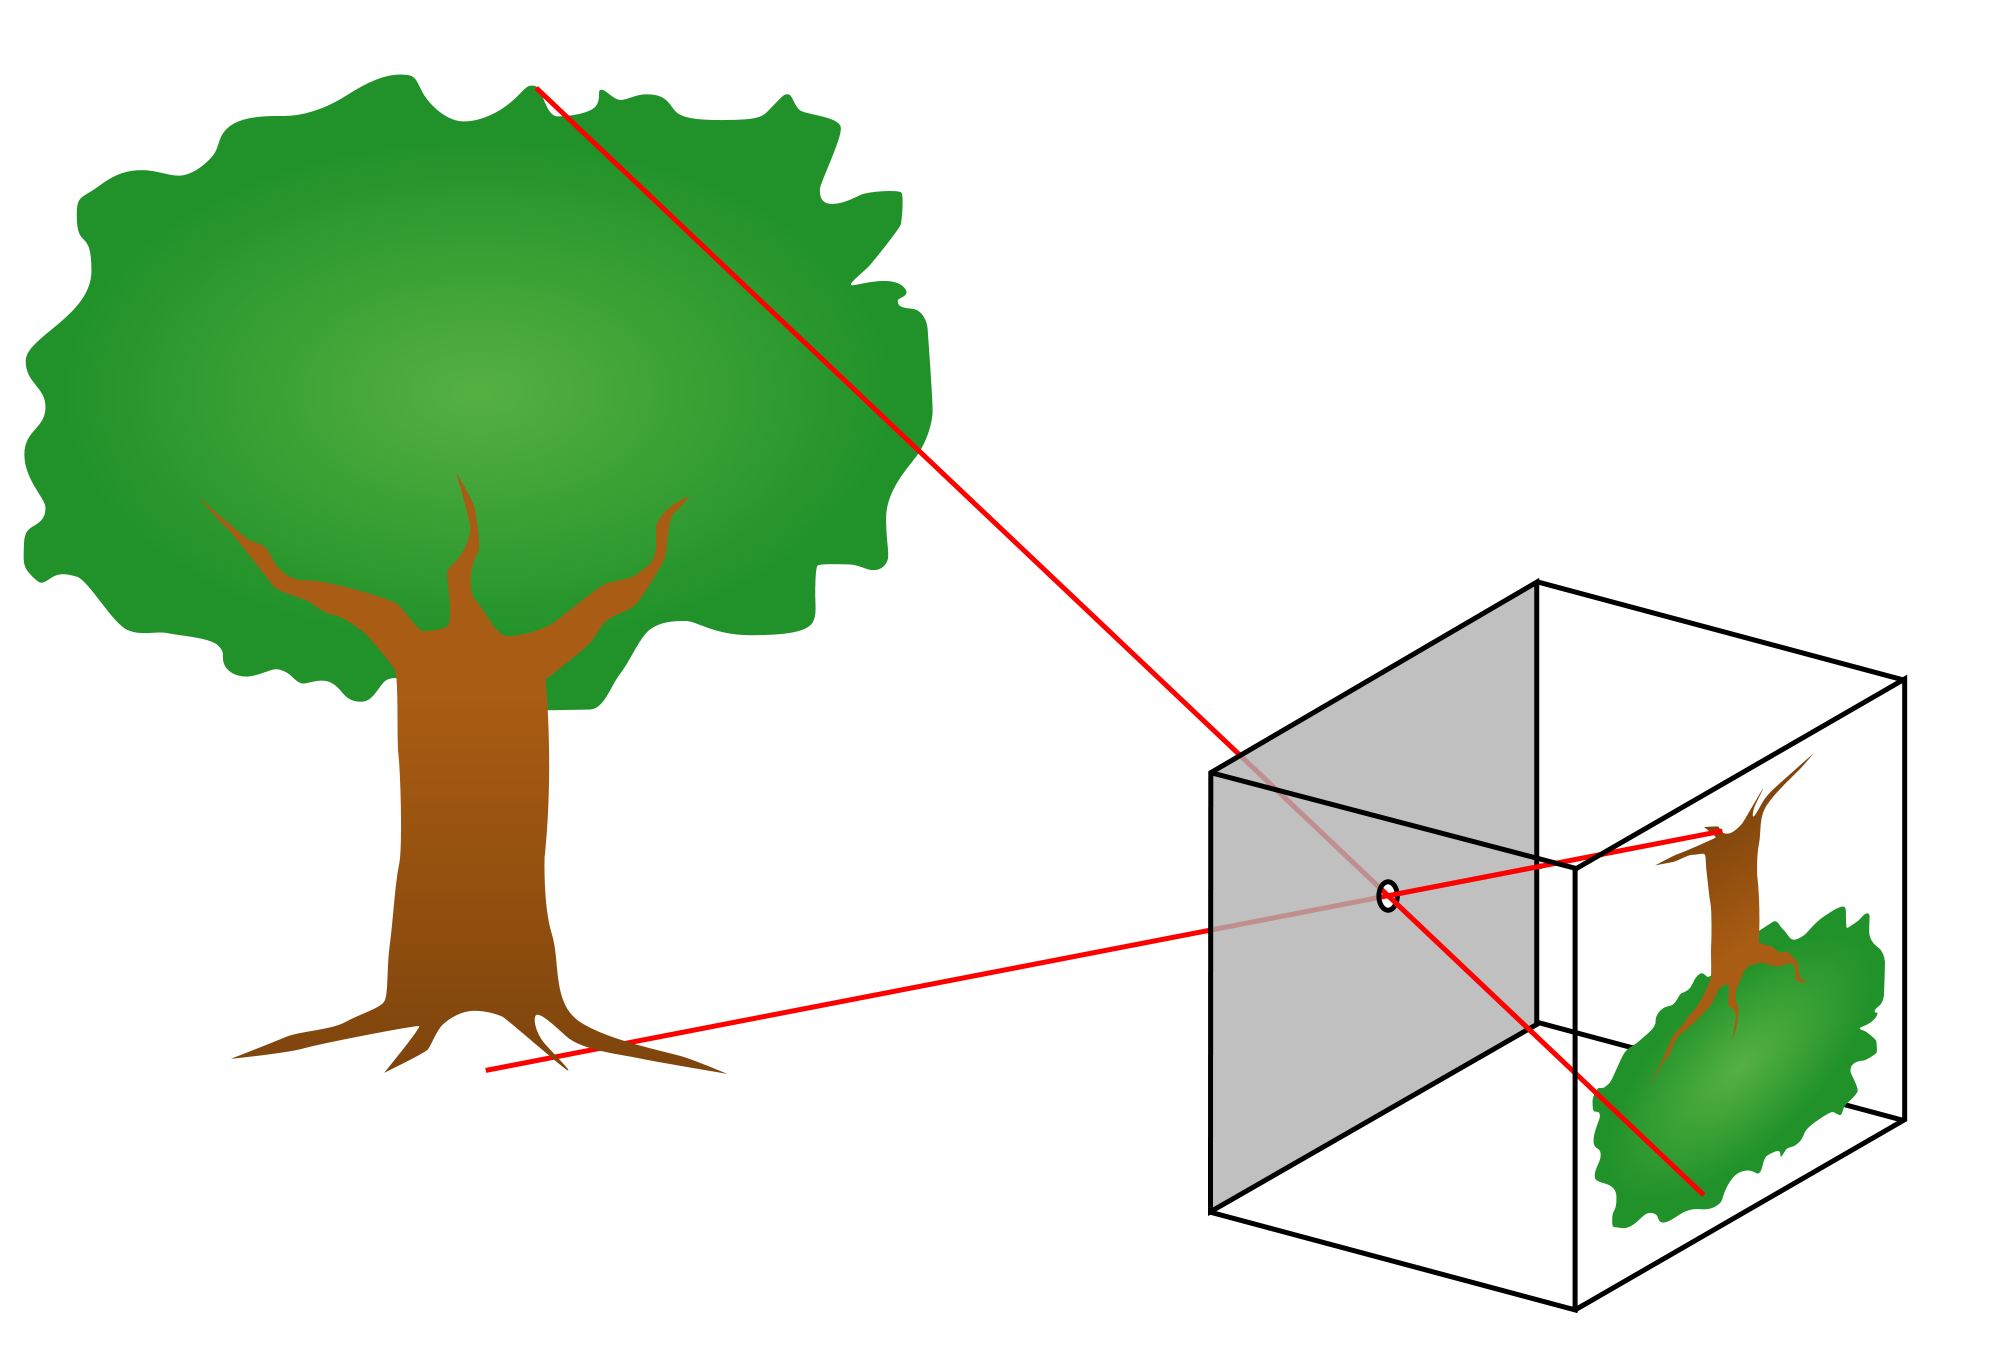
\includegraphics[width=\linewidth]{img/PinholeCam.png}
  \caption{ Pin hole camera model.}\label{fig:PanTiltRoll}
  \endminipage\hfill
\end{figure} 
 The pin hole model is commonly composed by box (or chamber) closed hermetically to light excepted by a small pin hole on the middle of front side. All the ray of light reflected by the object of the world and passing by the small hole are projected onto the back side of the box. Each rays of light passing by the hole are  projected on the plan (inside the box). This plan became the reversed image and can be recorded by a film or a sensor. 
 Due to the simplicity of the pin hole model (no lens, no mirror) the calibration and camera projection  estimation is simplified.\\
  Based on it the camera projection is dependent then few parameters intrinsic ( as focal length, sensor size,...) and extrinsic (as the position $x,y,z$ and orientation $\alpha,\beta,\gamma$) . 
  
 
\begin{figure}[t!]
\minipage{0.65\textwidth}
   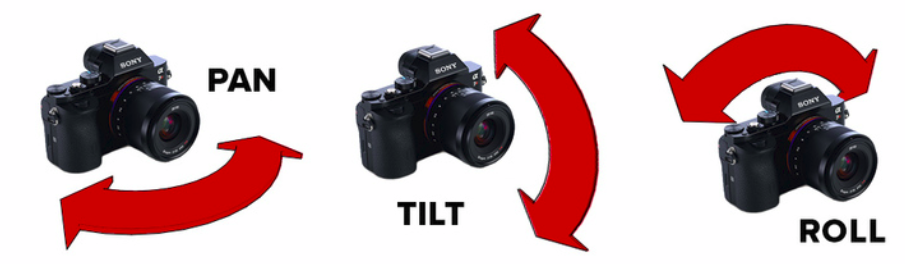
\includegraphics[width=\linewidth]{img/PanTiltRoll.png}
  \caption{ The rotation composed by 3 degrees of freedom on pan tilt roll$(\alpha,\beta,\gamma)$.}\label{fig:PanTiltRoll}
  \endminipage\hfill
\end{figure}

In fact the useful elements to define the projection of a camera perspective, can be stated as a set of parameters composed by :\\
\begin{itemize}
\item Three degrees of freedom of the sensor’s position: $(x, y, z)$;
\item Three degrees of freedom of the sensor’s orientation: the pan, tilt, and swing angles: $(\alpha,\beta, \gamma)$ 
\item Optical parameters including: the focal length $f$ of the lens, the sensor size $s$,  $ u_{0}$ and $v_0 $  which would be ideally in the centre of the image. $\sigma_{uv}$ represents the skew coefficient between the x and the y axis.
\end{itemize}
$s$ is composed by two element $Sw$ and $Sh$ for the size on width and height (also called scale factor).\\

The useful parameter of the camera can be formalized as a vector :
\begin{equation}\label{eq:v}
v=(x,y,z,\alpha ,\beta,\gamma,f,s,u_0,v_0,\sigma_{uv})
\end{equation}

Each element of the vector $v$ are necessary to compute the camera projection on to each individual point of the discretized floor. 
\iffalse 
To model the set of the cameras using the precedent notation, a set $V$ composed by $N$ cameras defined by $v$ noted:
\begin{equation}\label{eq:V}
\begin{split}
V= \{v_i\} \mbox{  , } \forall i=[1;N] \mbox{ , } N\in \mathbb{N}^*
\\
\mbox{ and } v_i= (x_i,y_i,z_i,\alpha_i ,\beta_i,\gamma_i,f_i,s_i,{u_0}_i,{v_0}_i,{\sigma_{uv}}_i)
\end{split}
\end{equation}
\noindent Where $N$ is the given number of cameras in the solution. Which is also the number of cameras in the set $V$. \\
Therefore, $V$ represent a camera networks and also a initial set of parameter for a set of cameras. $V$ can contain all the possibility, included the non-acceptable answer. A non acceptable  answer will be an answer with  doe's not respect the constraint of the problem.   
 \\ !!!!!!\\

%%%%%%%%%%%%%%%%%%%%%%%%%%%%%%%%%%%%%%%%%%%%%%%%%%%%  
  
 
    
The hole in the box is called the projection center. It is the point were each ray of light are crossing together.  \\
Based on this model, a 3D point $^CP=(^Cx,^Cy,^Cz,1)^T$ defined in the pin hole reference noted $ ^C\Re$ can be convert in to a 2D point  $^rp=(^ru,^rv,1)^T$ in the sensor reference (back side of the box) by using  the perspective projection model $pr() $: 
\begin{equation}
^rp=(^ru,^rv)= pr(^CP) \mbox{ with } \begin{cases} u= f.\frac{^Cx}{^Cz} \\  v= f.\frac{^Cy}{^Cz} 
\end{cases} 
\end{equation}
Where $f$ is the focal length (distance between the projection center and the photosensitive sensor )
the point $^rp$ is the projected point $^CP$ on the sensor. The sensor is composed by $sw$ pixel of width and $sh$  pixel of  heigh. To convert the coordinate $^rp$ of p in the pixel  that mean in the image reference $^i\Re$ : 
\begin{equation}
^ip=K. ^rp
\end{equation}
where $^ip$  is the point $p$ in the image reference composed by $(u,v) \in ^i\Re$ with $u$ and $v$ are  pixel coordinate. 


%Where $u_0$ and $v_0$ are the coordinate  of  the principal point of the image ( projection of the optic centre on to the image plan).  
%$k_u$ and $k_v$  are the magnification factors of the image on width and heigh. 

% resource http://ksimek.github.io/2013/08/13/intrinsic/
%https://jeux.developpez.com/tutoriels/OpenGL-ogldev/tutoriel-12-projection-perspective/
The cameras is called calibrated when the intrinsic parameters ($K$)are defined.  
 The intrinsic matrix $K$ is parametrized by Hartley and Zisserman and it is composed permit to represent the properties of the camera. To design the intrinsic matrix $K$ some part of the pin hole camera have to be defined :\\
  \begin{itemize}
  
 	\item $f$ is  the focal length. The focal length is the distance between the pinhole and the sensor (a.k.a. image plane)
  	\item $k_u et k_v$ are the magnification factors of the image on width and heigh ; related to the image sensor format%  les facteurs  aggrandisement de l'image 
  	\item $u_0 v_0$  are the coordinate  of  the principal point of the image ( projection of the centre optic on to the image plan)  %the les coordonnées de la projection du centre optique de la caméra sur le plan image 
  	%\item $s_uv$ qui traduit la non-orthogonalité potentielle des lignes et des colonnes de cellules électroniques photosensibles qui composent le capteur de la caméra. La plupart du temps, ce paramètre est négligé et prend donc une valeur nulle.\\
  	  \end{itemize}
		Once these elements are known the matrix $K$ can be designed :
	\begin{equation}
		K=
		\begin{pmatrix}
			k_u 	& 0 	& u_0 \\
			0 		& k_v	& u_1\\
			0 		&	0	& 1
		\end{pmatrix} .
		\begin{pmatrix}
			f 		& 0 	& 0  \\
			0 		& f		& 0  \\
			0 		&	0	& 1  
		\end{pmatrix} 
	\label{eq:K}
	\end{equation}
Finally, in order to estimate the positions of a 3D point in the pin hole camera reference $^C\Re$ in to the image reference $^i\Re$ 
$$
^ip=K.pr(^CP)
$$ 	  
 Parameter extrinsic (definition global) \\
  \begin{itemize}
 	\item$R_3x3$ = la matrice de rotation permettant de passer du repère lié à l'espace de travail au repère lié à la caméra\\
 	\item$t_x t_y t_z$ = les composantes du vecteur de translation permettant de passer du repère lié à l'espace de travail au repère lié à la caméra.\\
  \end{itemize}
 %Parameter utile pour notre cas de figure \\     fig : \ref{eq:V}\\
 
!!!!! the previous section can be largely (keep the basic introduction remove to be replace by ... !!!!!
\fi
%%%%%%%%%%%%%%%%%%%%%%%%%%%%%%%%%%%%%%%%%%%%%%%%%%%%%%%%%%%%%%%%%%%%%%%%%%%%%
\subsubsection{Coverage estimation in the literature}

%To estimate the coverage of a set of camera $V$  the cameras projection of each $v_i$ has to be computed individually.
 In order to compute the camera projection onto a grid the Pin Hole model is used with the parameters of the vector $v$.\\
 
The detail to estimate the camera projection on to the floor based on the pin hole model and the parameters $v$, has been detailed numerous times as in  [193* ,181*, 165*]. In [193* ,181*, 165*] the camera projection is used to estimate if a point is visible by a camera, for each point of the grid. These articles handles the classical camera projection (with the 6DoF in 193* and 5DoF in 181*),in order to estimate the 2D projection of the camera onto the floor. 
In the 193* the camera projection has been compute for several rotation and consider all the DoF. In this case the projection can have numerous shapes ( mostly parallelogram shape).
In 181* the  model of camera projection is begin to be simplified by assuming some of the parameter are fixed and do not need to be recompute at each time.  \\
In 165* the model of camera projection is used to compute one time for a fix pan and roll in order to have an coverage estimation usable in a 2D map. The camera projection is finally simplified by using a kind of triangle shape.
 Also Some of them [181*,165*,141*] include the object occlusion. To detected the part of the area occluded the solution commonly proposed( as in [181*]) is to check  if the line between the camera and the points cover by the camera is intersected by at least one object of the scene. 
  Despite the simplicity of the computation numerous operation have to be done to compute the camera projection onto the floor. \\

To go further other model inspired by the pin hole model have been used as [87* 141* 146* 194*]. These model are inherited for the camera projection and adapted to feet their problems. In order to simplify the estimate of the area covered by a set of cameras. \\
In [87*, 194*] the camera is considered to be placed on the floor with a fix pan (almost parallel to the floor). Therefore the camera projection is simplified by a isosceles triangle where the focal length shape of it.\\
Also in 141* the camera projection is simplified in order to have a kind of isosceles triangle shape with  
consider the depth of view of the camera.\\
In 146* thanks to a fix pan and focal length, the camera projection is simplified in order to estimate the size of the projection. In 146* once the size of cameras projection estimate the sweep is designed  in consequence, in order to minimize the overlap and  have full coverage of the area.   \\


One of the common point of the method present  ([87* 141* 146* 194*][22,33,193* ,181*, (165*)]) is the computation of a camera projection on to a grid. The computations necessary to estimate if a point of the area is cover are not considered as really greedy (in time). But have to be done to each point $g_j$ of the grid and for each camera $v_i$ of the network.
	\begin{equation} \label{eq:sum sum v g}
		\sum_{j=1}^{m}\sum_{i=1}^{n}f( v_i,g_j)
	\end{equation}
Where $n$ the number of cameras in the network; $m$ the number of  point in the grid; \\
The equation \ref{eq:sum sum v g} do not  take in account the occlusion by few obstacle $Obj$. If we add the occlusion  by $k$ object. 
	\begin{equation}
		 \sum_{k=1}^{k}\sum_{j=1}^{m}\sum_{i=1}^{n}f( v_i,g_j,Obj_k)
	\end{equation} 
 
The function  $f(...)$ in charge to compute a camera projection will be called for each camera, in order to evaluate the complete coverage of the area. This numerous call will greatly increase the time computation of the coverage.  It is even worst when numerous cameras projection ($n$)have to be computed at each turn of a long optimisation process.\\
In this condition the efficiency of the function $f()$ in charge then compute the coverage estimation is primordial.



\subsubsection{coverage estimation optimization}
Design a efficient cost function in order to reduce the time computation and estimate correctly the area covered is primordial for the optimisation process. \\
  The computation of the camera projection can be minimized with some basic assumption depending then the problem.\\
  
Considering our case, where a camera is fixed on a UAV with a looking direction orthogonal to the ground, without any rotation around the axis of $\alpha$ (pan) and $\beta$ (tilt). It is  possible to compute for a given altitude the area covered by one camera, based on the given parameters. Especially the focal $f$, the altitude of the cameras and the sensor size $s$. Where $s$ is composed of $Sw$ sensor size width and $Sh$, sensor size height ($s= [Sw ; Sh]$). \\

This model with no rotation around $\alpha$ and $\beta$ and a looking direction to floor permit to estimate the camera FoV projected onto the floor. The camera projection is always a rectangle as described in Figure \ref{fig:cam_proj}. To estimate the shape of the rectangle with is deduced from the ratio of $s$ and the size of this rectangle with is deduced from $ f ,s ,A$. Where $A$ is the altitude where $A$ is the difference between the camera and the grid position, considered to be equal to $z$.  

%\begin{equation}
%s= [Sw ; Sh]  %\mbox{   } Sw,Sh \in \mathbb{N} 
%\end{equation}
%
%\noindent Where $Sw$, sensor size width. \\
%Where $Sh$, sensor size height.
	\begin{equation} \label{eq:etaUpsilon}
 	 \begin{split}
		\eta = 2\times \tan^{-1} (\frac{Sw}{(2\times f)}  ) 
 	   \\
		\upsilon = (\frac{Sw}{Sh} )\times \eta
 	 \end{split}
	\end{equation}
Where $f$ is the focal length of the camera and 
$\eta$, $\upsilon$ are the horizontal and vertical camera fields of view.\\
Estimating the width and height of the rectangle projected on the ground depend on the altitude $A$ :
	\begin{equation}\label{eq:WrHr1}
		\begin{split}
    		Wr= 2\times A\times\tan \eta
    	    \\
    	    Hr= 2\times A\times\tan \upsilon
    	 \end{split}
	\end{equation} 
	\begin{figure*}[t!]
		\centering
		\minipage{0.85\textwidth}
  		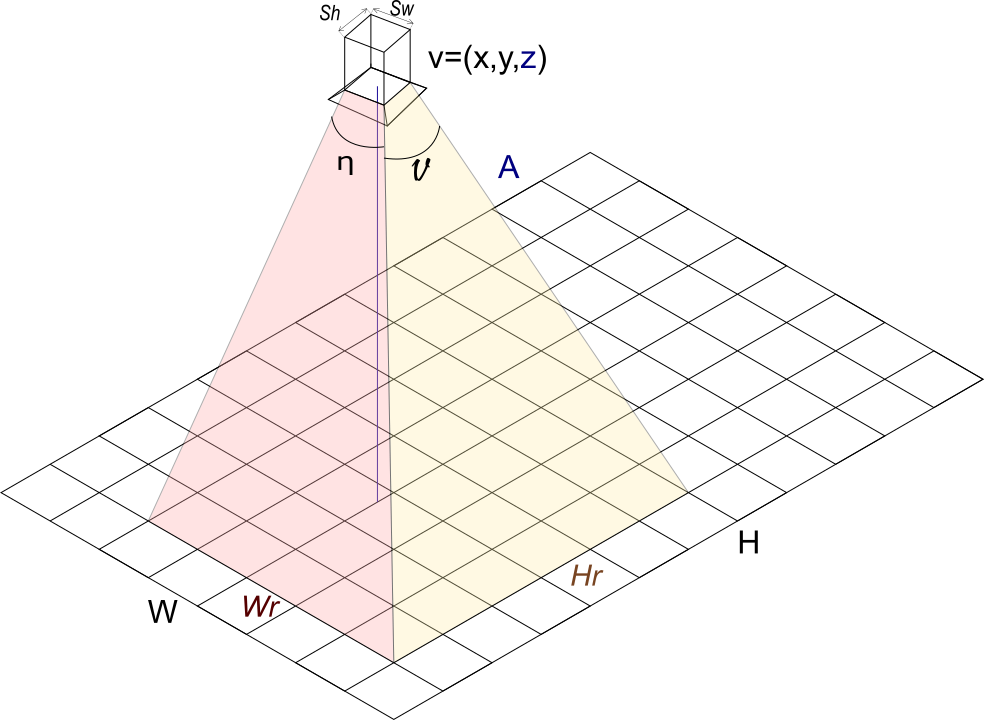
\includegraphics[width=\linewidth]{img/CamProject1Bis.png}
  
 	 	\endminipage\hfill\caption{Camera projection onto a grid. The grid is placed on the floor to discretize 	the area covered.}\label{fig:cam_proj}
	\end{figure*}

Therefore, the size of the rectangle projected onto the floor is $(Wr,Hr)$ for the width and height. The values of $Wr$ and $Hr$ are directly linked to the altitude of the camera. In the simple case and in the initialization, $A$ is equal to $z$ (see Eq:\ref{eq:V})  and $z$ is selected in a range given by the UAV or the user. \\
Once the couple $(Wr,Hr)$ as been computed for a $A=z$ it is easier to change the altitude of the camera. The rectangle projection will be affected in proportion.
	\begin{equation}\label{eq:A.coef}
		\begin{split}
 		   	f(A)= (Wr,Hr) \text{ based on eq \ref{eq:WrHr1}}\\
    		f(A.Coef)=f(z)= (Wr.Coef,Hr.Coef)      
    	 \end{split} 
	\end{equation}
Therefore, to any altitude $z$ is existing $A.Coef$ where the size of the camera projection onto the floor is $(Wr.coef, Hr.coef)$. Thanks to this the eq: \ref{eq:etaUpsilon} and eq: \ref{eq:WrHr1} have to be compute once  for a given focal length $f$  and sensor $s$ with an simple $A$. With this simple $Coef$ the size of camera projection can be easily simplified in order to limit the useless computation.

The model of camera projection is greatly simplified by the UAV assumption (no pan, no tilt and fix focal length). That permits to consider  the camera projection as a simple rectangle with a size directly related to the altitude (by using a simple coefficient $Coef$).\\
%The simplification by modelling all the cameras with a fix orientation and same ability (in order to have a rectangle projection onto the ground) 
All this simplification helps the cost function to be fast and efficient. \\

\subsection*{Parameter to optimize }\label{sec:parameterToOptimize}
% en raison de 
By dint of the simplification presented previously the useful parameter of the camera formalized as a vector can be simplified too.\\
To summarize, in order to compute the camera projection of one camera on to the floor. Where the floor is represented by a grid to discretize the area, and the camera is at altitude with a looking direction orthogonal to the floor.  Just few parameter are necessary  as showed in equation  \ref{eq:etaUpsilon} %{eq:WrHr1 , }
to \ref{eq:A.coef}. Thanks to that the equation (\ref{eq:v})  can be reduced with keeping only the position of the camera and the roll as:
	\begin{equation}\label{eq:v2}
		v=(x,y,z,\gamma )
	\end{equation}
	or also
	\begin{equation}\label{eq:v2}
		v=(x,y,A.coef,\gamma )
	\end{equation}

Also reducing the number of  parameter, passing to the equation \ref{eq:v2} to \ref{eq:v} are really usefully to the optimisation problem. The reduction of the number of parameter will  greatly affect the optimisation process.\\
 Indeed in addition to reduce the time computation, this simplification reduce the number of parameters to optimize.\\   

Until know the camera projection estimation as been addressed with only one camera. But we want to compute the coverage for a set of camera. \\
The solution is based on the previous camera projection estimation and adapt to the location of each camera (by translate the rectangle to have the center of it at the $x$ and $y$ position) and compute the occupation grid.\\

In order to win a bit of time each point of the grid already cover by a camera are note tested for the next cameras. This small modification will impact positively the computation time for the coverage estimation of a network of camera. That mean in the equation \ref{eq:sum sum v g} the value of $m$ decrease as $i$ increase. More exactly  the size of m decrease as  the area coverage increase.  
\\

\subparagraph*{ Representation of the parameters to optimize.\\ }
In order to represent correctly the set of camera with the useful parameter to compute the camera projection, the precedent notation can be adapted to have a set of $V$ composed by $N$ cameras defined by their parameters $v$:

	\begin{equation}\label{eq:V}
		\begin{split}
			V= \{v_i\} \mbox{  , } \forall i=[1;N] \mbox{ , } N\in \mathbb{N}^*
				\\
			\mbox{ and } v_i= (x_i,y_i,z_i,\gamma_i)
		\end{split}
	\end{equation}
\noindent Where $N$ is the given number of cameras in the network. Which is also the number of cameras in the set $V$. The coordinate of a camera $v_i$ with are the $i$th camera of the network is defined  with $x_i, y_i, z_i,$ for the given room and $gamma_i$ the roll rotation (portrait or landscape). The other  useful parameters are common to all the set $V$  for each problem.\\
Therefore, $V$ represent a solution. $V$ contain all individual positions and orientation of the set of cameras for a predefined focal length, sensor size and map depending then the problem.\\% wish also include the potential constraint as  some restriction on the map.\\
Obviously all the solution $V$ are not a "possible solution" for our problem. Some solution $V$ does not respect the set of $E$.

So that the $V$ should respect all the constraints of $E$ (see Eq.\ref{eq:Vs}). Where $E$ is the set of constraints. Among the constraint few of them was already disused, as the occlusion, the map restriction, the k-coverage, or some constraint more specific to the problems (as saw in chapter \ref{chap:stateOfTheArt}).\\
 The "possible solution" $Vs$ must take in consideration the set $E$ as :

\begin{equation}\label{eq:Vs}
Vs=V \mbox{ , iff } E(V)=\begin{cases}1, & \mbox{  iff } E_i(v)=1 \mbox{ , with } i=1...Nc \\ 0, & \mbox{otherwise} 
\end{cases} 
\end{equation}
Where $Nc$ is the number of constraints need to be satisfied to have an acceptable response.\\
That mean among all the possible combination of parameter $V$ only the one meet the constraint of the set $E$ in order to have an possible solution.  If we are considering  all the $V$ and all the $E$ as two subset $Vs$ is defined as $Vs=V\subset E$.\\ 

The problem of monitoring an area and more specifically the problem of area coverage may contain many constraints depending of the environment and the context, for example: the room shape and minimizing the altitude to have a best resolution, the orientation of the camera, the possible occlusion,... All this constraints are included in the set $E$. \\

\subsection{Constraint}

Make the exhaustive list of all the constraint for the problem of cameras positioning is not really interesting and almost impossible. The constraint can be numerous and depend mainly of the problem formulation and the context. Like that few of them was briefly introduced in the previous section as in chapter \ref{chap:stateOfTheArt}, section \ref{sec:coverageEstimation},...\\

The constraint considered in this work are : 
\begin{itemize}
	\item Fixes number of the cameras.
	\item Fixes parameters of camera.
	\item No rotation  on  $\alpha$ and $\beta$ (pan and tilt).
	\item Possible fixes altitude.
	\item Altitude boundary (not too hight, not too low).  	
	\item The map boundary (rigid rectangle).  
	\item Non rectangle map with possible hole.
	\item To have some fix cameras in the set. 

	\item The resolution.\\

\end{itemize} 
\subparagraph{Fixes number of the cameras.}
One of the first constraint is the fix number of cameras. This permits us to focus on the fine optimisation (as in  [22*] where both are tested). The number of camera is fixed at the beginning of the optimisation and no more camera will be added during the optimization process.  \\

\subparagraph{Fixes parameters of camera and no rotation.}
Fixes parameters of camera and no rotation  on  $\alpha$ and $\beta$, as introduce previously some parameters of the camera are fix (see \ref{sec:parameterToOptimize}). These constraints imposed by the use of an UAV is also an advantage for the optimization by simplify the coverage estimation and limit the number of parameters to optimize. The parameters are fixed at each beginning of the optimization.\\

\subparagraph{Fixes altitude.}
 The fix altitude is a constraint usable in order to limit the number of parameter to optimize. The use of this constraint is usable to reduce the Complexity (see \ref{sec:OptimizationComplexity}).  It is also useful for other assumption as a camera on the celling or for a submarine 66* \cite{66*}.\\

\subparagraph{The altitude boundary.}
 When the altitude is not fix  some limit must be fixed to avoid the extremely high and low altitude. The highest altitude will be fix depending then the UAV ability and local law. The lowest altitude have to be fix for the safety of the user under the UAV.  
In practice the boundary of the $z$ is defined  with 
 \begin{equation}\label{eq:boundaryZ}
   \inf z\leq A.Coef\leq \sup z  
 \end{equation} 
 Where $\sup z$ is the maximal altitude of the camera and $\inf z$ the minimum altitude. $A$ is the fix altitude  of a camera where the camera projection has been computed with $A=z$ with only $coef$  vary as introduced in Equation \ref{eq:A.coef}. \\ 
 
 \subparagraph{The map boundary.}
 The map boundary is a constraint similar then the altitude boundary. Despite the shape of the map for an area to cover some maximum boundary can be done. In fact for any shape as complex as it, it is  possible to  encapsulated in a rectangle. The rectangle map boundary is defined by a width $W$ and height $H$. The boundary on $x$ and $y$ are :
 \begin{equation}
  \begin{array}{lcl}
  	0\leq x\leq W \\ 0\leq y\leq H 
  \end{array} 
 \end{equation}  
 
By associating the altitude boundary (from Eq\ref{eq:boundaryZ}), a cube boundary limit the position of the cameras in the 3 dimensional space. 
\begin{equation}\label{eq:3dBoundary}
  \begin{array}{lclcl}
  	0\leq x\leq W \\ 0\leq y\leq H  \\ \inf z\leq A.Coef\leq \sup z  
  \end{array} 
 \end{equation} 
 
 \subparagraph{Non rectangle map with possible hole.}
Despite the rectangle boundary of the area, the map to cover can be much more complex and can take any kind of shape. The shape of the area can be composed by hole. The figure \ref{fig:boundaryMap} illustrate the map complexity. The black part of the map are the zone with are out. That mean these sub-parts have not interest to be covered.
 \begin{figure}[t!]
\minipage{0.85\textwidth}
   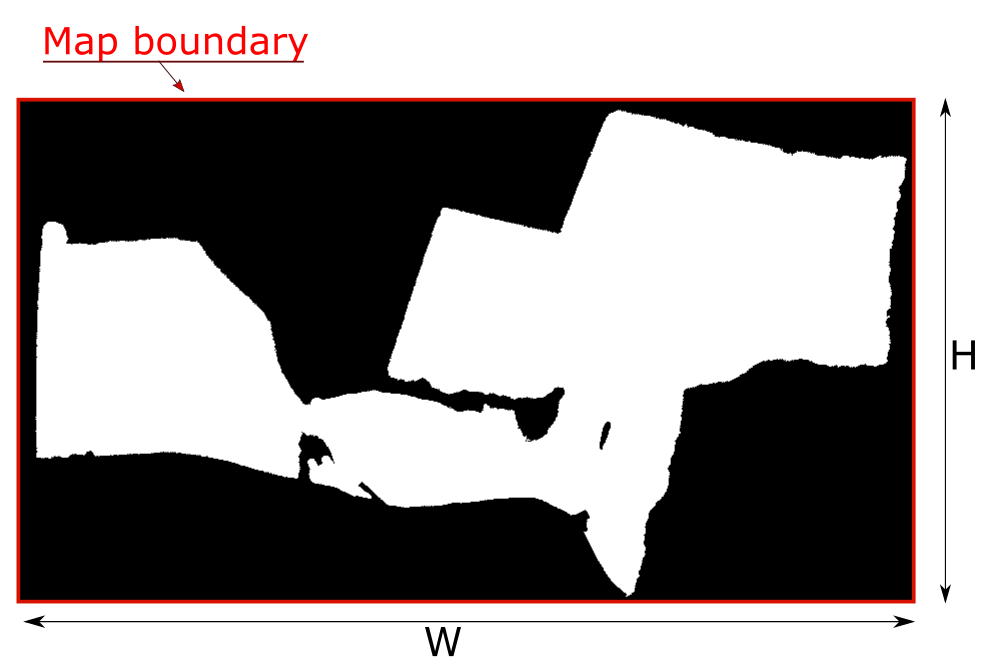
\includegraphics[width=\linewidth]{img/BoundaryMap2.png}
  \caption{Map to cover with the map boundary in red (W and H size) in black the sub-part have no interest to  be covered.   
}\label{fig:boundaryMap}
  \endminipage\hfill
\end{figure}
To take in account this constraint the gird have been designed with removing some of this points.
The grid $G$ is reduced in order to have only the points in the white sub-part. 
Concretely this implementation is easier for the complex map and have also some advantage. \\
Among the advantage the flexibility. The grid customization  allow the optimization to try some exotic solution, with example the camera on the black sub-part or  in a border of it.  Obviously  the exotic solution with a cameras position on the black side does not increase the coverage rate  but if the optimisation converge correctly no camera will be on the the black sub-part of the map (or small part of it).\\

\subparagraph{Some fix cameras in the set.}
To have some fix camera in the set, is an optional constraint. This allow to have few manual cameras position from an user or other algorithms.
One case can be to have some specific area as the entrance where have to be surveyed.  
To implement this constraint the solution applied during experiment (presented later) is to adapt the map by remove the point of the grid $G$ cover by the sub-set of fix cameras.\\

\subparagraph{The resolution.}
The resolution of the images is related then the sensor size (in px) and  the distance between the camera and the object filmed. In our case the sensor size is fixed by the properties of the camera mounted on the UAV and the object filmed is the floor of the area to cover. In this case the distance between the camera and floor is the altitude. \\
The resolution constraint have to maximize the resolution. In order to maximize the resolution during the optimization the altitude criteria is modified in order to be the lower possible.\\
During the optimization a trade off between the altitude (and the related resolution) and the coverage rate have to be done $\min{\frac{\sum^n_{i=1}{A.coef_i}}{n}}$ and the coverage rate . In order to manage this trade off, the average altitude of the cameras position is included in the cost function (*******ajouté lien ver la partie******). 
 

 
Among the constraints listed different priority and restriction exist. Indeed the constraint can be considered in 2 sub-class. 
 Some of the constraints presented are called "Hard constraint". \\
 The hard constraint limit the possible solution by do not allowing to have a answer $Vs$ with does not respect it. This hard constraint is directly used during the optimisation process to prohibit any solution to be out of this boundary. This hard constraint have to be integrate in the optimization process in order to cannot  generate a solution with does not respect it. \\ 
 For example the 3D boundary as defined in Equation \ref{eq:3dBoundary} is an hard constraint. Each cameras position must be inside the 3D boundary.\\
 
 In the other case some constraint can be considered as "Soft constraint".\\ 
 The soft constraints is to minimize the set of error. If a small constraint is not fully respected the solution can be considered as acceptable and this small amount of error does not affect so much the final answer. \\
 The soft constraint leave the possibility during the optimization to do some mistake in order to learn about it.  
 If the soft constraint is noted $\epsilon'$ and the hard in order to have constraint are noted $\epsilon''$ like that the constraint set is $E=\epsilon'+\epsilon''$.
 \begin{equation}
 	\max f(Vs) -\epsilon'  \mbox{  } \forall Vs \subset \epsilon''
 \end{equation}
  \begin{equation}
 	\max f(Vs) - \min \epsilon'  \mbox{  } \forall Vs \subset \epsilon''
 \end{equation}

.\\............................\\
 cost function  
 $\max{\frac{\sum^m_{i=1}{g_i}}{m}}$, where $g_i = 1$ when the point of the grid $G$ coverer by the set of cameras


%%The use of an UAV to cover an area allow the simplification of coverage computation as well as the numbers of parameters to optimize.
%% !!!!
%%Thanks to the simplification of the problem due to the used of an uav the parameters to optimize can be reduced. (as in eq: \ref{eq:v}
%%Thanks to the simplification the element to optimize for an efficient coverage can be limited to pass from Eq. (\ref{eq:v}) to  Eq.(\ref{eq:v2}) as shown: 
%%\begin{equation}\label{eq:v2}
%%v=(x,y,A,\gamma )
%%\end{equation}
 %%%%%%%%%%%%%%%%%%%%%%%%%%%%%%%%%%%%%%%%%%%%%%%%%fin de la camera pin hole explication%%%%%%%%%%%%%%%%%%%%%%%%%%%%%%%%%%%%%%%%%%%%%%%%%%%%%%%%%  
%    
%In the following part a vision sensor is employ to acquire the image of area to control. The vision sensor may be a common camera with different parameter as:
% \begin{itemize}
% \item Every camera has a position  in  $(x, y, z)$;
% \item Every camera  has an orientation composing to 3 degrees of freedom  pan$(\alpha$),  tilt$(\beta)$, roll$(\gamma)$, see Figure \ref{fig:PanTiltRoll}.
% \item Every camera have different optical parameters and the helpful to take in consideration for coverage estimation is the focal length $f$ and the sensor size $s$(based on the formulation of Chrysostomou et al[82]). 
% \end{itemize}


 
%%%%%%%%%%%%%%%%%%%%%%%%%%%%%%%%%%%%%%%%%%%%%%%%%%%%
 \subsection{Optimization complexity} \label{sec:OptimizationComplexity}
 
%To cover an area with a certain amount of sensor many solutions can be possible.
In spite of the simplification presented before, the problem stay complex. There exist many position for each camera to cover an area with certain amount of sensors. This number of position can be estimate as follow.\\   
Each camera defined by the position on $x, y, z $ and $ \gamma$ can be set anywhere in the search space  named $Sp$ : 
\begin{equation}\label{eq:SearchSpace}
 Sp=(W\times H \times ( \max(A)-\min(A)) \times \gamma )  Sp \in E 
\end{equation}
Where $W$ and $H$ are the size as width and height of the area to cover, $\max(A)-\min(A)$  is the possible altitude. The $\gamma$ is to define the roll, as the rectangle projection is horizontal or vertical ( landscape or portrait). The search space $Sp$ allows to take in consideration some strong constraint $E$ like the boundary of the area or the restriction in the degree of freedoms.

The Problem of the search space is the propensity to increase rapidly as the area grow. This phenomena is accentuate for a set of $N$  waypoints.
%It is possible to express the size of the search space as a succession of product for estimate the number of feasible position on $x, y, z $ and $ \gamma$ for each combination of the set cameras : 
%\overset{N}{\underset{Sp}{e}
 \begin{equation} \label{eq:Combinaison}
 \begin{pmatrix} N \\ Sp \end{pmatrix}  = \frac{Sp!}{N!(Sp-N)!} = |Vs|
 \end{equation} 
 Where $|Vs|$ is the number of possible solution for a set of $N$ cameras. %$|Vs|$ is the 
 %  \begin{equation} \label{eq:SearchSpace}  \sum_{n=1}^N \sum_{x=1}^{W} \sum_{y=1}^{H} \sum_{z=1}^{)} \sum_{\gamma=1}^{2}Pc_i  - \sum_{k=1}^{E}Pc_i=Vs  \end{equation}
 In fact the size of the search space ( as Eq. \ref{eq:SearchSpace}) associate to the set of $N$ cameras (as Eq.\ref{eq:Combinaison}) make a exponential number of possible solution depending mainly then the size of the area and the number of the waypoints in the network. 
 Obviously in view of this behaviour the use of a deterministic solution based on a heuristic does not seem to be a good answer to have a efficient solution. In addition the number of possible solutions $|Vs|$ makes the computation of an optimal almost impossible due to the numerous local minima. This kind of problem can not be used with an algorithm dedicate to the research of global optimal solution but need to be used with an algorithm focusing of optimize the solution and return a acceptable solution.
 !!!! to continue !!!!

\section{From Journal Jirs}
%%%%%%%%%%%%%%%%%%%%%%%%%%%%%%%%%%%%%%%%%
\iffalse 
\section*{ to delete}
 In the following article a vision sensor is employ to acquire the image of area to control. The vision sensor may be a common camera with different parameter as:
% \begin{itemize}
% \item Every camera has a position  in  $(x, y, z)$;
% \item Every camera  has an  orientation  composing  to 3 degrees of freedom  pan$(\alpha$),  tilt$(\beta)$, roll$(\gamma)$, see Figure \ref{fig:PanTiltRoll}.
% \item Every camera have different optical parameters and the more important to take in consideration  for coverage estimation is the focal length $f$ and the sensor size $s$(based on the formulation of Chrysostomou et al[82]). 
% \end{itemize}
% 
%\begin{figure}[t!]
%\minipage{0.65\textwidth}
%   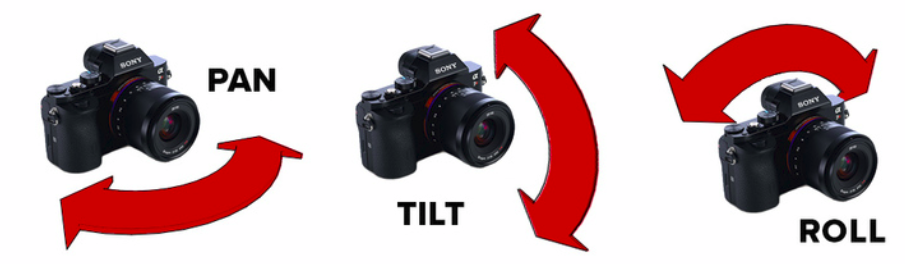
\includegraphics[width=\linewidth]{img/PanTiltRoll.png}
%  \caption{ The rotation composed by 3 degrees of freedom on pan tilt roll$(\alpha,\beta,\gamma)$.}\label{fig:PanTiltRoll}
%  \endminipage\hfill
%\end{figure}

In fact the different elements useful to define the cameras, can be stated as a set of parameters composed by :\\
\begin{itemize}
\item Three degrees of freedom of the sensor’s position: $(x, y, z)$;
\item Three degrees of freedom of the sensor’s orientation: the pan, tilt, and swing angles: $(\alpha,\beta, \gamma)$ 
\item optical parameters including: the focal length $f$ of the lens and the sensor size $s$.
\end{itemize}
All the parameter of the camera can be formalized as a vector :
\begin{equation}\
v=(x,y,z,\alpha ,\beta,\gamma,f,s)
\end{equation}
To model the set of the cameras using the precedent notation, a set $V$ composed by $N$ cameras defined by $v$ noted:
%In order to cover an area a set of cameras (defined by their parameter $v$ ) are used. This set of camera is defined by $V$:
%The problem of coverage is to optimize a set of parameters $v$, composed like in Eq.(\ref{eq:v}) for every cameras. 

\begin{equation}
\begin{split}
V= \{v_i\} \mbox{  , } \forall i=[1;N] \mbox{ , } N\in \mathbb{N}^*
\\
\mbox{ and } v_i= (x_i,y_i,z_i,\alpha_i ,\beta_i,\gamma_i,f_i,s_i)
\end{split}
\end{equation}
\noindent Where $N$ is the given number of cameras in the solution. Which is also the number of cameras in the set $V$. \\
Therefore, $V$ represent a solution. But all the solution $V$ are not a possible solution for our problem. 

So that the $V$ should respect all the constraints of $E$ (see Eq.\ref{eq:Vs}). Where $E$ is the set of constraints (describe later).
%are not  noted as $Vs$ if   all the parameter of $v$ satisfies all the constraints of $E$.
\begin{equation}
Vs=V \mbox{ , iff } E(V)=\begin{cases}1, & \mbox{  iff } E_i(v)=1 \mbox{ , with } i=1...Nc \\ 0, & \mbox{otherwise} 
\end{cases} 
\end{equation}
Where $Nc$ is the number of constraints need to be satisfied to have an acceptable response.\\
The problem of monitoring an area and more specifically the problem of area coverage may contain many constraints depending of the environment and the context, for example: the room shape and minimizing the altitude to have a best resolution, the orientation of the camera, the possible occlusion,... All this constraints are included in the set $E$. \\

\subsubsection{Coverage estimation} \label{sec:coverageEstimation}
Considering the case where the camera is fixed on a UAV with a looking direction is orthogonal to the ground without any rotation from $\alpha$ and $\beta$, it is  possible to compute for a given altitude the ground area cover by one camera based on the given parameters of $v$, especially the focal $f$, the sensor$s$ and the altitude of the camera. Using this model with no rotation around the $\alpha$ and $\beta$ the camera projection onto the floor is always a rectangle projection as described in Figure \ref{fig:cam_proj}. The size of this rectangle is deduced from $ f ,s$ and the altitude $z$. 
\begin{equation}
s= [Sw ; Sh]  %\mbox{   } Sw,Sh \in \mathbb{N} 
\end{equation}

\noindent $Sw$, sensor size width. \\
$Sh$, sensor size height.
\begin{equation} 
  \begin{split}
	\alpha H = 2\times \tan^{-1} (\frac{Sw}{(2\times f)}  ) 
    \\
	\alpha V = (\frac{Sw}{Sh} )\times \alpha H
  \end{split}
\end{equation}
Where $f$ is the focal length of the vision sensor and 
$\alpha H$, $\alpha V$ are the angle of view horizontally and vertically from the camera.\\
To estimate the width and height size of the projected rectangle onto the ground depending on the altitude $A$:
\begin{equation}\label{eq:WrHr}
	\begin{split}
    	Wr= 2\times A\times\tan \alpha H
        \\
        Hr= 2\times A\times\tan \alpha V
     \end{split}
\end{equation} 
Therefore a rectangle with the size $(Wr, Hr)$ for the width and height, can represent the projected  camera field of view. The size of $Wr$ and $Hr$ is directly linked to the coefficient $A$ ( for altitude). In the simple case $A $ is equal to  $z$ and $z$ is selected in a range given by the UAV ability or the user. The simplification by modelling all the cameras with a fix orientation and same ability (in order to have a rectangle projection onto the ground) helps the cost function to be fast and efficient. 

Thanks to the simplification the element to optimize in order to have an efficient coverage can be limited to pass from Eq. (\ref{eq:v}) to  Eq.(\ref{eq:v2})  as presented: 
\begin{equation}\label{eq:v2}
v=(x,y,z,\gamma )
\end{equation}

\subsection{ Waypoint positioning formulation. }\label{WaypointPositiongForm}

The goal of waypoint positioning is to manage the positioning of the fixed numbers of vision sensors in order to maximize the visual coverage. Indeed before finding the position some assumptions should be made.
%Indeed to use the evolutionary algorithm to optimize the problem of coverage is essential to define the objectives and  design the cost function. 
In the following, the coverage term denotes all parts of the floor visible by at least one camera. 
 Therefore, the problem is formulated as follows:
\begin{itemize}
\item [-] Maximization of the coverage with a fixed number of cameras.
\item [-] Minimization of the constraints, for example, the complex shape of the area, the bound of the area, the altitude of the UAV,...
\end{itemize}

The problem needs to be formalized in order to clearly identify the complexity of the waypoint positioning.
In this section, the waypoint to the position is considered as a set of camera views. \\
The positions of the cameras views have to limit the number and the size of black holes to be exploitable. The black holes are the area not covered by the camera views. 
To do so a precise estimated of the part covered by the system of camera views is elemental.
\\To know if the area is covered by a minimum of one camera, the techniques calls for representing the area by numerous placed points at the height of the ground. This point can be distributed “randomly” or uniformly on the ground as presented by Van Den Hengel et al \cite{83*} or it can be distributed by following a basic pattern  such as a grid shape.  Let $G$ be the grid map of the area to cover and $G_i$ is the $i^{th}$  point of the grid: %The grid noted $G$ with $G_i$ is the specific point $i$ of the grid is noted by 
\begin{equation}
G=\begin{bmatrix}
 g_1 ...g_i ... g_m
\end{bmatrix}  ,\mbox{ with }  m\in \mathbb{N}.
\end{equation}

\noindent Where $m$ is the number of points in the grid. The size of the grid is also an important factor affecting the precision, and computing complexity. If the value  of $m$ is too small, the coverage will be badly estimated. That will also affect the pose of the vision sensors. A value too high for $m$ will increase the complexity of the coverage estimate in terms of computation time and size of the search space and it will affect the camera pose. \\
The value of $m$ should be chosen carefully, depending on the ability and the number of the cameras, the area size and the goal. \\
%The solution the more used to design the $G$ stay the occupation grid. 
The occupation grid has been widely employed and easily implemented for designing $G$  \cite{8*,137*,164*,141*,151*}.
Every point of the grid $G$ should be covered at least by one camera. Consequently, a binary list of points is created to count the covered part of $G$ which is noted as $Pc$.
\begin{equation}\label{eq:Pci}
Pc_i= \begin{cases} 1, & \mbox{if } g_i\mbox{ is covered by $k$ cameras} \\ 0, & \mbox{otherwise}  \end{cases}
 \mbox{ , }k\geq 1
\end{equation}
  


\noindent Where $k$ is the number of cameras used to cover the point $g_i$ (of the grid $G$). In our case $k=1$ but can be easily adapted according to the need. $k=1$ is to specify the area that has to be covered with as little overlap as possible.\\
$Pc$ is the set of points covered by at least $k$ vision camera views, as in Eq.\eqref{eq:Pci}. \\

The vision sensor or, more precisely, camera contains many parameters:
\begin{itemize}
\item Each camera has a position  in  $(x, y, z)$ in the Cartesian system.
\item Each camera  has an  orientation with 3 degrees of freedom, pan$(\alpha$),  tilt$(\beta)$ and roll$(\gamma)$.
\item Every camera has different optical parameters. Among these parameters, two of  most interesting are, the focal length $f$ and the sensor size $s$. 
\end{itemize}

%\begin{figure}[t!]
%\centering
%\minipage{0.65\textwidth}
% 
%   \includegraphics[width=\linewidth]{fig3.png}
%  \label{fig:pan_tilt_Roll}
%  \endminipage\hfill
%  \caption{ The  rotation composed by 3 degrees of freedom on pan,  tilt, roll for $(\alpha,\beta , \gamma)$.}
%\end{figure}
In fact, the different elements used to define the camera poses, can be stated as a set of parameters.\\
 
\begin{equation}\label{eq:v}
v=(x,y,z,\alpha ,\beta,\gamma,f,s)
\end{equation}
To cover an area, a set of cameras (defined by their parameter $v_i$ ) are used. This set of cameras is defined by $V$:
%The problem of coverage is to optimize a set of parameters $v$, composed like in Eq.(\ref{eq:v}) for every cameras. 


\begin{equation}\label{eq:V}
\begin{split}
V= \{v_i\} \mbox{  , } \forall i=1,...,N \mbox{ , } N\in \mathbb{N}^*
\\
\mbox{ and } v_i= (x_i,y_i,z_i,\alpha_i ,\beta_i,\gamma_i,f_i,s_i)
\end{split}
\end{equation}
\noindent Where $N$ is the given number of cameras in the solution, which is also the number of cameras in the set $V$. \\
Therefore, $V$ is a potential solution. However, all the potential solutions $V$ are not a possible solution to our problem. To become a feasible solution the $V$ should respect all the constraints of $E$ (see Eq.\ref{eq:Vs}). Where $E$ is the set of constraints (described later).
%are not  noted as $Vs$ if   all the parameter of $v$ satisfies all the constraints of $E$.
\begin{equation}\label{eq:Vs}
Vs=V \mbox{ , iff } E(V)=\begin{cases}1, & \mbox{  iff } E_i(v)=1 \mbox{ , with } i=1...Nc \\ 0, & \mbox{otherwise} 
\end{cases} 
\end{equation}
Where $Nc$ is the number of constraints needed to be satisfied to have an acceptable response.\\
%The problem of monitoring an area and more specifically the problem of area coverage may contain many 
The constraints depend on the environment and the context; for example: the room shape and the altitude minimization for good resolution, the orientation of the camera, the possible occlusion (obstacle), few fixes of camera position, priority area, strongly restricted zone, relief, etc. All these constraints are included in the set $E$. \\
$Vs$ is a solution fulfilling all the constraints of $E$. The difference between $V$ and $Vs$ is the respect of the constraints $E$.%, a solution $V$ can be rejected as non possible solution (as out of the search space) when $Vs$ can be efficient enough to be the final solution.
The set of solutions $Vs$ can be formulated with $ Vs\subset V  $ and $ Vs\subset E$, where $V$ is a set for the search space and $E$ is the set of constraints with $V \cap E = Vs$. 
\fi
%%%%%%%%%%%%%%%%%%%%%%%%%%%%%%%%%%%%%%%%%%
%Concerning the case of the camera is fixed UAV without any rotation from $\alpha$ and $\beta$  the following assumption may consider as true. 
%Considering the case where the camera is fixed on UAV with a looking direction is orthogonal to the ground without any rotation from $\alpha$ and $\beta$ . 
%The projection model of the camera is not explicitly taken into account, but the ground-projected visual field of view instead, as described in Figure \ref{fig:cam_proj}, with the focal $f$ and the sensor specificity $s$ are known and fixed. Therefore a rectangle can represent the projected field of view of the cameras. This simplification help the cost function to be fast and efficient. 
%%%%%%%%%%%%%%%%%%%%%%%%%%%%%%%%coverage estimation%%%%%%%%%%%%%%%%%%%%%%%%%%%%%%%%%%%%
\subsubsection{Coverage estimation.} \label{sec:coverageEstimation}



%%%%%%%%%%%%%%%%%%%%%%%%%%%%% FIN coverage estimation%%%%%%%%%%%%%%%%%%%%%%%%%%%%%%%%%


 
